\subsection{Inteligencia Artificial}

La Inteligencia Artificial es la inteligencia que se produce por máquinas. Una máquina "inteligente" ideal es un agente adaptable que percibe su entorno y realiza acciones que maximizan sus posibilidades de éxito, según \parencite{tec_poole1998machinelearning}. Este término se usa cuando una máquina imita las funciones "cognitivas" que conectan a los humanos con otras mentes.

Se han seguido cuatro perspectivas a lo largo de la historia de la humanidad: dos se centraron en el comportamiento humano y dos se centraron en la racionalidad. El enfoque centrado en el comportamiento humano se basa en la ciencia empírica, es decir, experimentos que confirman y refutan hipótesis. Este método surgió de la prueba de Alan Turing en 1950. El matemático inglés famoso creó una prueba basada en la incapacidad de un computador para distinguir entre seres humanos y entidades inteligentes indiscutibles. Se dice que es una "máquina inteligente" si puede distinguir y superar la prueba mientras que el ser humano no puede. Por lo tanto, el computador debería tener las siguientes habilidades: procesamiento de lenguaje natural para comunicarse, representación del conocimiento describiendo lo que percibe de su entorno, razonamiento automático utilizando la información que ha procesado en su interior, y aprendizaje automático para adaptarse a nuevos eventos. Se dice que se está realizando la Prueba Global de Turing si el evaluador decide incluir una señal de video para evaluar la percepción de la computadora. Además de las cuatro capacidades mencionadas anteriormente, la computadora debe tener capacidades de visión computacional y robótica para percibir objetos y manipularlos. La mayoría de estas seis habilidades o áreas de conocimiento son parte de la Inteligencia Artificial, según \parencite{bk_russell2004intart}.

El enfoque racional, por otro lado, utiliza una combinación de ingeniería y matemáticas basadas en las "leyes del pensamiento". Estas provienen de la Grecia antigua, donde grandes filósofos como Aristóteles intentaron codificar la "manera correcta de pensar", lo que llevó al estudio de la lógica más adelante. En el siglo XIX, se desarrollaron programas que podían resolver problemas de notación lógica. Por lo tanto, la práctica logística en el ámbito de la Inteligencia Artificial se enfoca en crear sistemas inteligentes que tengan estas habilidades. El término "agente racional" proviene de todo lo mencionado anteriormente sobre el enfoque racional y se refiere a aquellos que actúan con el fin de lograr el mejor resultado, o el mejor resultado esperado, en caso de incertidumbre. Finalmente, la Inteligencia Artificial y sus fundamentos se derivan de muchas ciencias, como la economía, la neurociencia, la psicología, la ingeniería computacional, la teoría de control y la cibernética, y hasta la lingüística, además de la filosofía y las matemáticas según \parencite{bk_russell2004intart}.

Sin embargo, ¿cómo se origina este extenso análisis de la Inteligencia Artificial? Dos investigadores de neurociencia colaboraron para crear el primer trabajo de Inteligencia Artificial en 1943, basándose en el análisis formal de la lógica proposicional de Russell y Whitehead, la teoría computacional de Turing y la fisiología y funcionamiento fundamentales de las neuronas en el cerebro. Warren McCulloch y Walter Pitts propuso un modelo basado en neuronas artificiales, en el que cada una de ellas se identificaba como "activada" o "desactivada". La estimulación generada por una cantidad suficiente de neuronas cercanas resultó en el primer tipo. Por ejemplo, demostraron que una red de neuronas conectadas podría calcular cualquier función de cómputo y que las estructuras de red sencillas eran capaces de implementar todos los conectores lógicos. Después de seis años, Donald Hebb propuso una regla para actualizar la intensidad de las conexiones entre las neuronas, la cual se conoce como la "regla de aprendizaje Hebbiano" y sigue siendo válida hasta la actualidad. En el taller de Dartmouth de John McCarthy, Allen Newell y Herbert Simon crearon un programa de computación que tenía la capacidad de pensar de forma no numérica y estaba basado en el Teórico Lógico. Sin embargo, este artículo no fue publicado en la revista textit Journal of Symbolic Logic. Sin embargo, los trabajos de los colaboradores que participaron en ese taller se mantuvieron durante 20 años más, y McCarthy fue quien introdujo el término "Inteligencia Artificial" en este campo \parencite{bk_russell2004intart}.

En los años 80, la IA comenzó a entrar en la industria, especialmente en las empresas más grandes de los países desarrollados, a través de grupos especializados para la realización de investigaciones de sistemas expertos, así como en la construcción de computadoras cada vez más poderosas y capaces de resolver tareas más complejas.

En la actualidad, la inteligencia artificial tiene una amplia gama de aplicaciones, incluida la minería de datos, el procesamiento de lenguaje natural, la robótica y los videojuegos. Se pueden encontrar otras ramas dentro de él, como el aprendizaje automático, la visión computacional, etc.

\subsection{Aprendizaje Automático}
El Aprendizaje Automático es una rama de la Inteligencia Artificial que busca técnicas que las computadoras pueden aprender a través de encontrar algoritmos y heurísticas para convertir muestras de datos en programas sin necesidad de hacerlas, según \parencite{bk_russell2009intart}. Sus algoritmos están compuestos por una variedad de tecnologías, incluido el procesamiento de lenguaje natural, las redes neuronales y el aprendizaje profundo. Estas tecnologías se utilizan en el aprendizaje supervisado y no supervisado, ambos que se basan en lecciones de información actuales. La premisa fundamental del aprendizaje automático es crear algoritmos que puedan recibir datos de entrada y usar análisis estadístico para predecir una salida mientras se actualizan las salidas a medida que se adquiren nuevos datos según \parencite{bk_alpaydin2014ml}.

Se puede clasificar en cuatro tipos principales de la siguiente manera según el objetivo que se desea alcanzar mediante el uso de ML:
\begin{itemize}
	\item \textbf{Aprendizaje supervisado}: El aprendizaje supervisado se ganó su nombre porque los científicos de datos actúan como una guía para enseñarle al algoritmo las conclusiones a las que debe llegar. Es similar a la forma en que un estudiante aprende aritmética básica de un maestro. Este tipo de aprendizaje requiere datos etiquetados con las respuestas correctas que se esperan del resultado del algoritmo. Para problemas de clasificación y regresión, el aprendizaje supervisado demostró ser preciso y rápido según \parencite{bk_zambrano2018supnosup}.
	
	Los dos tipos de aprendizaje supervisado son:

	\begin{itemize}
		\item \textbf{La Clasificación}: es la predicción del valor categórico de salida que permite dividir los datos en "clases" específicas. La clasificación se puede usar para varios propósitos, como determinar el clima, determinar si un correo electrónico es spam o no o identificar tipos de animales después de recibir una educación adecuada, un conjunto de datos con etiquetas de imágenes que incluyen la especie y algunas identificaciones características, según \parencite{bk_zambrano2018supnosup}.
		\item \textbf{La Regresión}: es un tipo de problema en el que la predicción de un valor de respuesta continua es necesaria, como los precios de las acciones y la vivienda, según \parencite{bk_zambrano2018supnosup}.
	\end{itemize}

	Por lo tanto, funciona modelando las relaciones y dependencias entre las características de entrada y la salida de predicción objetivo, lo que permite predecir los valores de salida para nuevos datos utilizando las relaciones que aprendió de conjuntos de datos anteriores, según \parencite{bk_alpaydin2014ml}.

	\item \textbf{Aprendizaje no supervisado}: Por otro lado, el aprendizaje no supervisado se asemeja más a lo que algunos expertos llaman inteligencia artificial real: la idea de que una máquina puede aprender a identificar patrones y procesos complejos sin la supervisión de humanos. Cuando los expertos no saben qué buscar en los datos y los datos en sí no incluyen objetivos, este método es particularmente útil. La agrupación de k-means, el análisis de componentes principales e independientes y las reglas de asociación según \parencite{bk_zambrano2018supnosup} son algunos de los muchos casos de uso del aprendizaje automático no supervisado.
	
	\begin{itemize}
		\item \textbf{Agrupación K-means}: es un tipo de problema en el que cosas similares están agrupadas, como se muestra en la Figura 16. Comparte el mismo concepto con la clasificación, pero no se proporcionan etiquetas, por lo que el sistema entenderá los datos y los agrupará. Un uso de esto sería agrupar los artículos y las noticias según su género y contenido, según \parencite{tec_sancho2018supnosup}
	\end{itemize}
	
		\begin{figure}[h]
		\begin{center}
			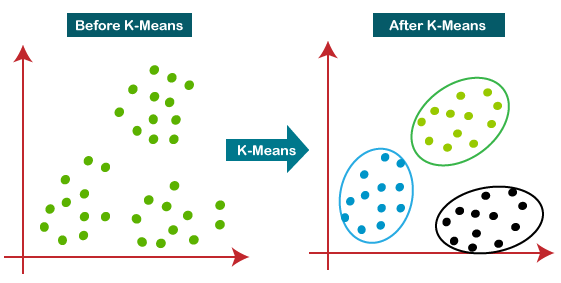
\includegraphics[width=0.75\textwidth]{2/figures/kmeans.png}
			\caption[Funcionamiento del algoritmo de K medias]{Funcionamiento del algoritmo de K medias.\\
			Fuente: \cite{tec_sancho2018supnosup}. \citetitle{tec_sancho2018supnosup}.}
			\label{2:fig3}
		\end{center}
	\end{figure}
		
	Debido a su complejidad y dificultad de implementación, este tipo de aprendizaje automático no se utiliza tan frecuentemente como el aprendizaje supervisado, a pesar de que abre las puertas a la resolución de problemas que los humanos normalmente no abordarían, según \parencite{tec_sancho2018supnosup}

	\item \textbf{Aprendizaje semisupervisado}: Hasta el momento, todos los datos enviados han sido etiquetados con el resultado deseado o no han sido etiquetados en absoluto. El aprendizaje automático semisupervisado utiliza ambos. El costo de etiquetar es bastante alto en muchas situaciones prácticas y, en el caso de grandes conjuntos de datos, se vuelve aburrido y requiere mucho tiempo. Además, proporcionar demasiados datos etiquetados puede hacer que el modelo tenga sesgos humanos. A pesar de que los datos sin etiquetar son desconocidos para la red, ofrecen información útil sobre los parámetros del grupo objetivo. que conduce a la conclusión de que se puede mejorar la precisión del modelo al incluir datos sin etiquetar y, al mismo tiempo, ahorrar tiempo y dinero en su construcción. Por ejemplo, la clasificación de páginas web, el reconocimiento de voz o la secuenciación genética pueden usar aprendizaje automático semisupervisado. En esos casos, los científicos de datos pueden acceder a grandes cantidades de datos sin etiquetarlos, y la tarea de etiquetarlos todos llevaría mucho tiempo, según \parencite{bk_zambrano2018supnosup}.

	Se puede comparar estos tres tipos de aprendizaje automático para el mismo uso, como clasificación, utilizando los datos recopilados hasta ahora:

	\begin{itemize}
		\item \textbf{Clasificación supervisada}: el algoritmo clasificará los tipos de páginas web según las etiquetas proporcionadas desde el principio, según \parencite{bk_zambrano2018supnosup}.
		\item \textbf{Agrupación no supervisada}: el algoritmo buscará patrones y características que ayudan a agrupar páginas web en grupos, según \parencite{bk_zambrano2018supnosup}.
		\item \textbf{Clasificación semi no supervisada}: identificará varios grupos de páginas web utilizando los datos etiquetados, luego utilizará los datos no etiquetados para establecer los límites de esos grupos de páginas web y buscar otros tipos que posiblemente no aparezcan en los datos etiquetados, según \parencite{bk_zambrano2018supnosup}.
	\end{itemize}
	

	\item \textbf{Aprendizaje por refuerzo}: junto con el aprendizaje supervisado y no supervisado, es el aprendizaje por refuerzo. Como se muestra en la Figura 17, se compone de cinco componentes principales: el agente, el entorno, el estado, la acción y la recompensa. Utilizando su interacción con el entorno, RL busca maximizar la recompensa y reducir el riesgo. El algoritmo RL (también conocido como agente) mejorará el entorno a intervalos regulares experimentando varios estados potenciales. Los agentes seleccionarán automáticamente el comportamiento ideal para maximizar el rendimiento. La retroalimentación, también conocida como recompensa, es lo que permite al agente mejorar su comportamiento, según \parencite{bk_sutton2018rl}.
	
	\begin{figure}[h]
		\begin{center}
			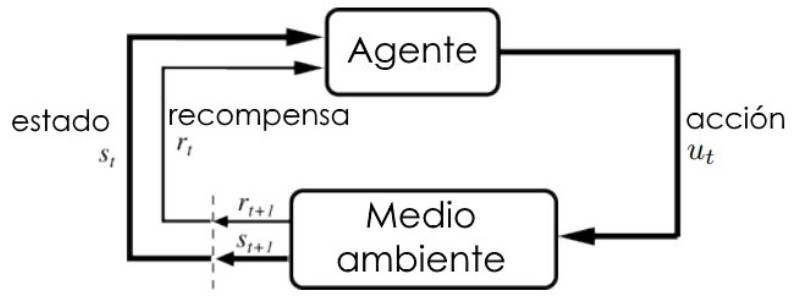
\includegraphics[width=0.60\textwidth]{2/figures/aprendizaje_refuerzo.jpg}
			\caption[Componentes del Aprendizaje por Refuerzo]{Componentes del Aprendizaje por Refuerzo.\\
				Fuente: \cite{bk_sutton2018rl}. \textit{Finite Markov Decision Processes}. (p. 48)}
			\label{2:fig4}
		\end{center}
	\end{figure}
	
\end{itemize}

\subsection{Aprendizaje Profundo}

Desde que llegó la Inteligencia Artificial hace un tiempo, tiene una amplia gama de aplicaciones y se divide en muchas ramas, como se menciona en \parencite{gl_sas_deeplearning}. El aprendizaje profundo es un subconjunto del aprendizaje automático, que es en sí mismo un subcampo de la IA. La Figura 18 es una representación visual de la relación entre AI, ML y DL.

\begin{figure}[!ht]
	\begin{center}
		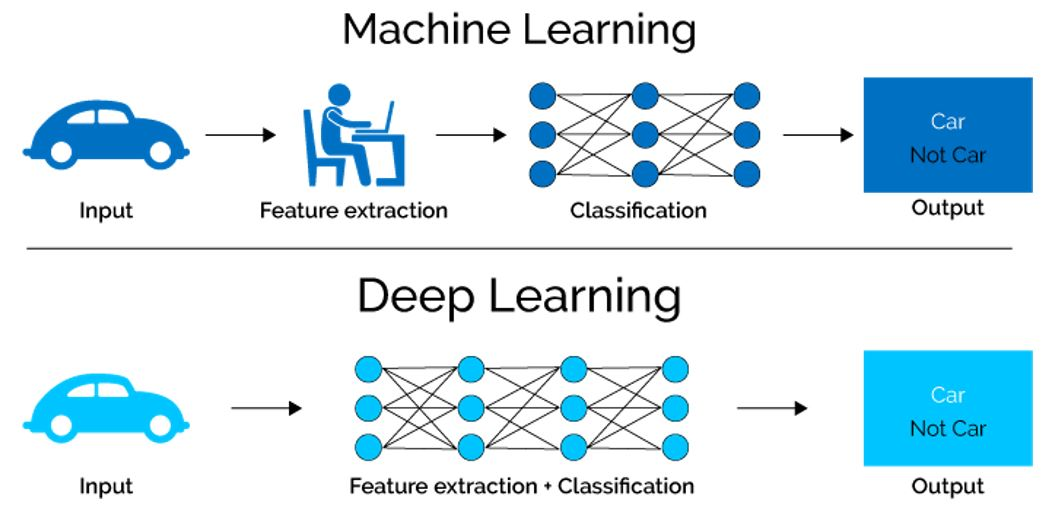
\includegraphics[width=0.50\textwidth]{2/figures/deeplearning_machinelearning.jpg}
		\caption[Relación entre IA, ML y DL]{Relación entre IA, ML y DL.\\
		Fuente: \cite{tec_cook2018deeplearning}. \textit{Most Popular 20 Free Online Courses to Learn Deep Learning}.}
		\label{2:fig5}
	\end{center}
\end{figure}

El aprendizaje profundo no solo permite representar datos de la manera correcta, sino que también permite que la computadora aprenda programas informáticos de varios pasos al incluir el concepto de profundidad en sus modelos. Como se muestra en la Figura 19, cada capa de representación puede interpretarse como el estado de la memoria de la computadora. Las computadoras interpretan las imágenes como una colección de valores de píxeles que representan escenas de nuestra realidad. Según \parencite{tec_cook2018deeplearning}, identificar un objeto o mapear su identidad a partir de esos valores es una tarea difícil para las máquinas y puede resultar casi imposible cuando se intenta aprender este mapeo directamente.

\begin{figure}[!ht]
	\begin{center}
		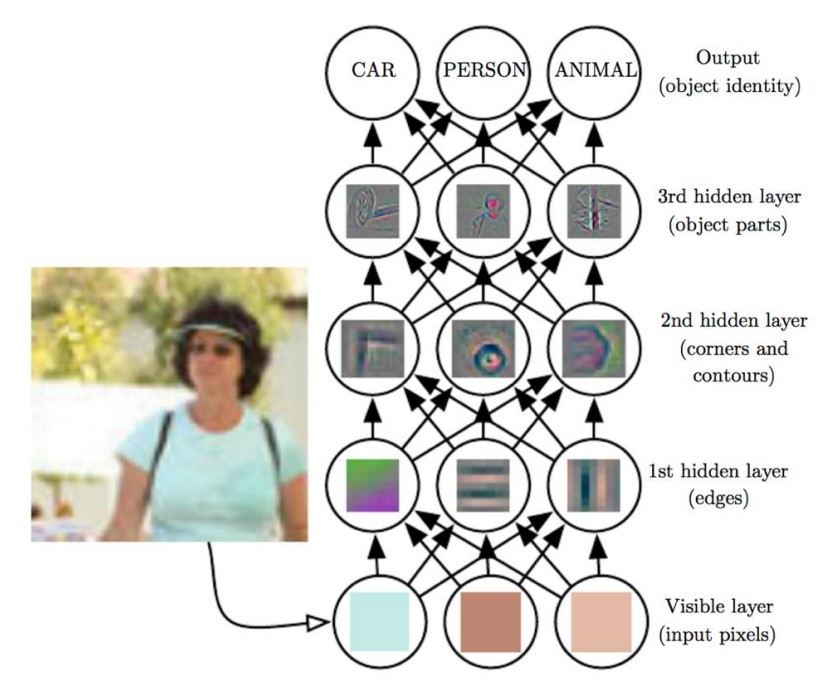
\includegraphics[width=0.70\textwidth]{2/figures/deeplearning_machinelearning2.jpg}
		\caption[Ilustración de un modelo de aprendizaje profundo]{Ilustración de un modelo de aprendizaje profundo.\\
		Fuente: \cite{tec_cook2018deeplearning}. \textit{Most Popular 20 Free Online Courses to Learn Deep Learning}.}
		\label{2:fig6}
	\end{center}
\end{figure}


\subsection{Aprendizaje Profundo Multimodal}
El Aprendizaje Profundo Multimodal se basa en la explotación de representaciones latentes en las redes neuronales profundas para agrupar diferentes modalidades (como audio, imágenes, texto, videos, etc.) o múltiples tareas (como predicción, clasificación, series de tiempo, entre otros), como se muestra en la Figura \ref{2:fig6} \parencite{bk_deng2018deeplearningnlp}.

\begin{figure}[!ht]
	\begin{center}
		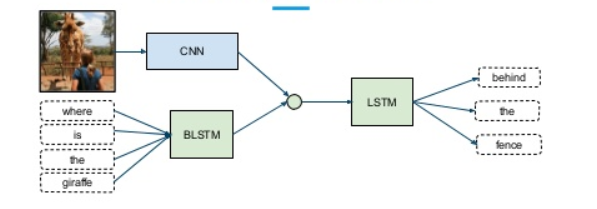
\includegraphics[width=0.85\textwidth]{2/figures/multimodal_network.png}
		\caption[Un modelo multimodal que combina imágenes y texto]{Un modelo multimodal que combina imágenes y texto.\\
		Fuente: \cite{tec_nishida2015multimodal}. \textit{Multimodal gesture recognition using multi-stream recurrent neural network}.}
		\label{2:fig7}
	\end{center}
\end{figure}

Los modelos de este tipo pueden realizar inferencias más sólidas porque las señales de diferentes modalidades llevan información complementaria sobre diferentes aspectos de un objeto, evento o actividad. Actualmente se utilizan técnicas multimodales como fusión temprana y tardía, fusión de modelos, ensamblado de modelos y redes neuronales profundas. Las características combinadas que se modelan en grupo para la toma de decisiones y, debido a que pueden recopilar información útil y hacer predicciones colectivamente, se denominan "enfoques aditivos", según \parencite{tec_liu2018multideeplearning}.

Trabajar con modelos multimodales no solo mejora las redes neuronales, sino que también permite una mejor extracción de características de todas las fuentes para realizar predicciones a mayor escala, según \cite{tec_baheti2020introduction_mdl}. Uno de los principales beneficios es que los datos, que provienen de diferentes fuentes, brindan información que se complementa entre sí y revela patrones ocultos que no se pueden ver cuando se trabajan individualmente las modalidades, mejorando así la predicción.

\begin{figure}[!ht]
	\begin{center}
		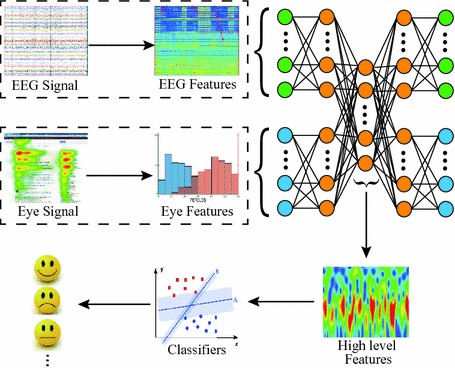
\includegraphics[width=0.79\textwidth]{2/figures/multimodal_deep_learning_example.jpg}
		\caption[Un modelo multimodal para las señales de electroencefalografía y de ojo]{Un modelo multimodal para las señales de electroencefalografía y de ojo.\\
		Fuente: \cite{tec_baheti2020introduction_mdl}. \textit{Introduction to Multimodal Deep Learning}.}
		\label{2:fig7}
	\end{center}
\end{figure}

\subsection{Inteligencia Artificial Generativa}

La inteligencia artificial generativa es el campo de la ciencia que estudia cómo crear inteligencia totalmente automatizada. Esto contrasta con el campo de la inteligencia artificial moderna, que investiga cómo los humanos comprenden y construyen la inteligencia. La construcción manual es lo que hacen los investigadores, pero la parte "por humanos" de la definición de IA suele ser una variable oculta en la construcción de los sistemas de IA contemporáneos. Aunque la diferencia puede parecer sutil, incluso innecesaria, la construcción automatizada requiere una perspectiva completamente nueva, que no está disponible en la literatura sobre IA actual. No importa si los humanos comprenden cómo funcionan los mecanismos internos de una máquina en la Inteligencia Artificial Generativa, aunque podría ayudar a los investigadores en su búsqueda de la creación de máquinas inteligentes. Lo que importa es que la máquina pueda controlar y dirigir el proceso de creación de estructuras internas en la dirección deseada. Es como criar hijos: los seres humanos no son conscientes de los procesos mentales, pero interactúan con sus hijos en un nivel diferente al hablar de sus sustratos neuronales. En lugar de eso, utilizan una variedad de máquinas clasificadoras para diferenciar los comportamientos positivos de los negativos, que podrían ser beneficiosos para el niño cuando sea mayor. Los castigos corporales, los institutos educativos, los medios de comunicación y otros lugares son algunos de los usos de estas máquinas clasificadoras, según \parencite{th_zant2010genai}

A continuación, ofrecemos una variedad de categorías de modelos de inteligencia artificial generativa.

\begin{itemize}
	\item \textbf{Modelos de difusión}: crean nuevos datos iterando cambios aleatorios controlados en una muestra de datos previa. Empezan con los datos originales y luego agregan cambios sutiles, también conocidos como ruido, que hacen que gradualmente pierdan la similitud con el original. Este ruido se controla minuciosamente para garantizar que los datos generados sigan siendo consistentes y realistas. El modelo de difusión invierte el proceso después de agregar ruido en varias iteraciones. Como se muestra en la Figura 22, la eliminación de ruido inversa crea una muestra de datos nueva que se asemeja a la original, según \parencite{tec_amaz2023iagen}.
	
	\begin{figure}[!ht]
		\begin{center}
			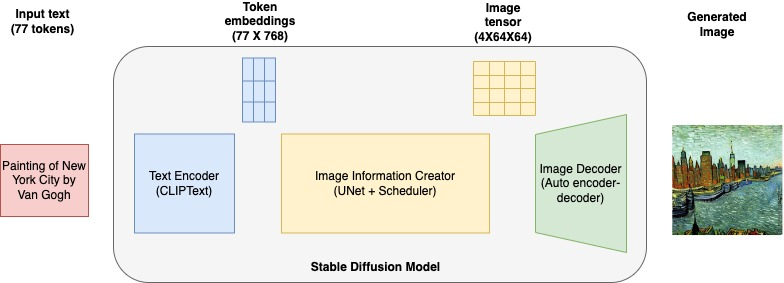
\includegraphics[width=0.85\textwidth]{2/figures/modelosdedifusion.jpg}
			\caption[Modelos de difusión]{Modelos de difusión.\\
			Fuente: \cite{tec_amaz2023iagen}. \citetitle{tec_amaz2023iagen}.}
			\label{2:fig8}
		\end{center}
	\end{figure}

	\item \textbf{Redes generativas adversativas}: compiten con dos redes neuronales. La primera red, también conocida como generador, agrega ruido aleatorio para crear muestras de datos falsas. La segunda red, conocida como discriminador, ayuda a distinguir entre los datos reales y falsos generados por el generador. El generador mejora continuamente su capacidad de generar datos realistas, mientras que el discriminador mejora su capacidad de distinguir entre lo real y lo falso. Hasta que el generador produzca datos tan persuasivos que el discriminador no pueda diferenciarlos de los datos reales, este proceso adversativo termina, según \parencite{tec_amaz2023iagen}.

	\item \textbf{Autocodificadores variacionales}: aprenden sobre el espacio latente, una pequeña representación de datos. La representación matemática de los datos se conoce como espacio latente. Puede verse como un código único que representa los datos en función de cada característica. Por ejemplo, cuando se estudian los rostros, el espacio latente contiene números que representan la forma de las orejas, los pómulos, la nariz y los ojos. Las dos redes neuronales utilizadas por los VAE son el codificador y el decodificador. Para cada dimensión del espacio latente, la red neuronal del codificador mapea los datos de entrada a una media y una varianza. crea una muestra aleatoria utilizando la distribución normal gaussiana. Este ejemplo es un punto en el espacio latente, y como se puede ver en la Figura 23, representa una versión comprimida y simplificada de los datos de entrada, según \parencite{tec_amaz2023iagen}.
	
	\begin{figure}[!ht]
		\begin{center}
			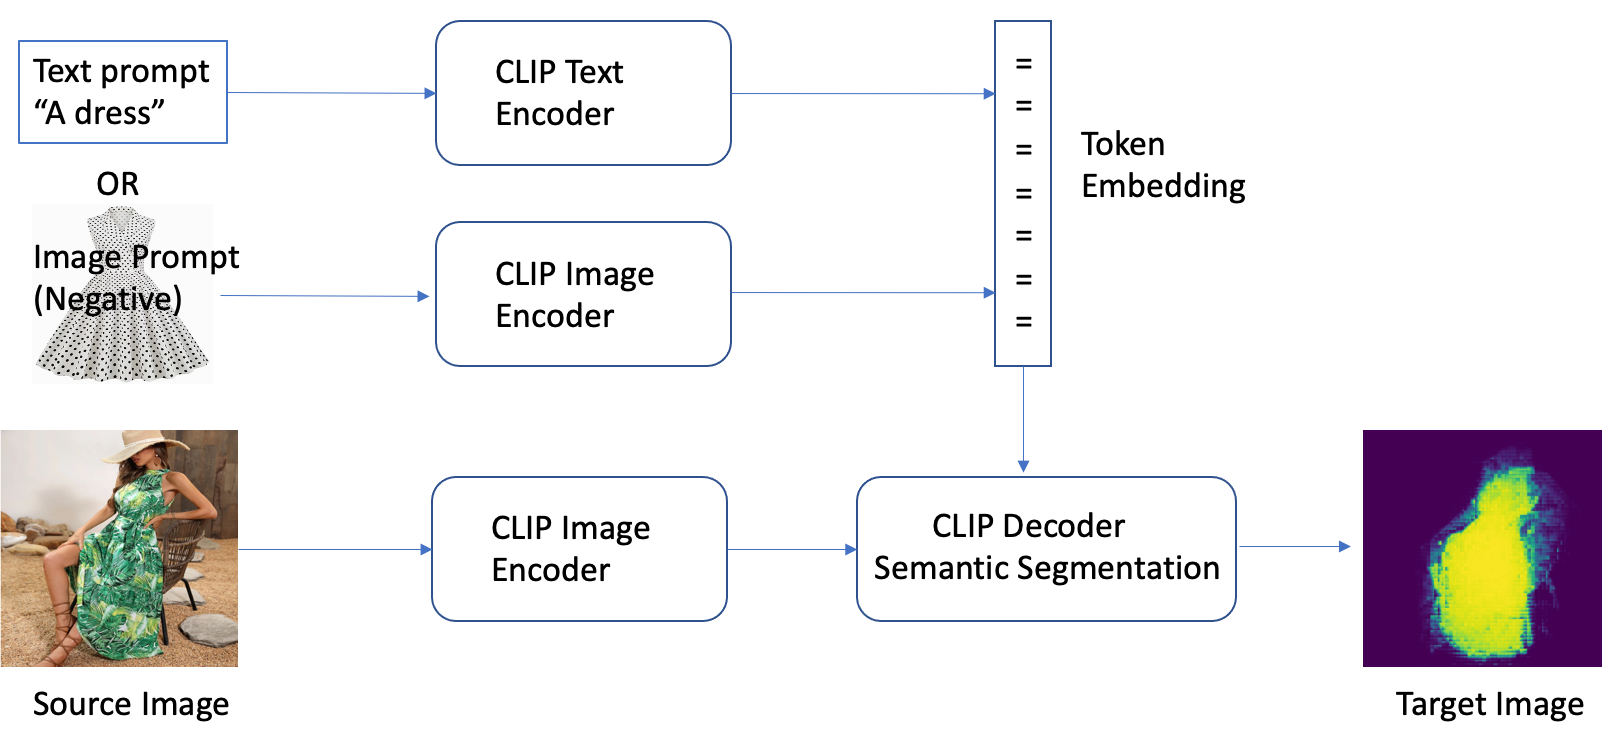
\includegraphics[width=0.85\textwidth]{2/figures/autocodificadoresvariacionales.png}
			\caption[Autocodificadores variacionales]{Autocodificadores variacionales.\\
			Fuente: \cite{tec_amaz2023iagen}. \citetitle{tec_amaz2023iagen}.}
			\label{2:fig9}
		\end{center}
	\end{figure}
\end{itemize}


\subsection{Modelos de Predicción}

Se utilizan modelos de datos estadísticos para predecir el comportamiento futuro. Se recopilan datos actuales e históricos, se crea un modelo estadístico, se hacen predicciones y se validan a medida que se obtienen más datos. Los modelos predictivos tienen como objetivo evaluar la probabilidad de que un agente muestre un comportamiento específico en el futuro a través del análisis de su desempeño anterior. Además, la búsqueda de patrones ocultos está incluida como dice \parencite{gl_gartner2019pm}.

\subsection{Análisis de Datos Espaciales}

El análisis espacial es una colección de técnicas y modelos que utilizan explícitamente referencias espaciales para cada valor de datos u objeto especificado en el sistema en estudio. Los métodos de análisis espacial necesitan hacer suposiciones o basarse en datos para describir las relaciones espaciales o interacciones espaciales entre casos. Los resultados de cualquier análisis espacial no son iguales cuando se reordenan la distribución espacial de valores o se reconfigura la estructura espacial del sistema. \parencite{bk_haining2003spdat}

Al realizar un análisis estadístico, es necesario tener en cuenta muchas características de los datos espaciales. El análisis de la dependencia espacial es crucial para el análisis de datos espaciales y central, por ejemplo, para realizar predicciones espaciales o especificar diseños de muestreo. Sin embargo, concentrarse demasiado en este aspecto de los datos espaciales puede llevar al analista a ignorar otras cuestiones. Por ejemplo, el impacto de una partición de área en la precisión de un estimador o el conjunto más amplio de supuestos y efectos de los datos que determinan si un modelo puede considerarse apropiado para el propósito previsto. Por lo tanto, el análisis de datos espaciales es una rama del análisis de datos más amplio. \parencite{bk_haining2003spdat}

Existe, por lo tanto, un papel importante para las áreas de la teoría estadística desarrolladas para manejar otros tipos de datos no espaciales, al definir las habilidades y conceptos necesarios para realizar un análisis adecuado de datos espaciales. Se mantiene un vínculo con el cuerpo más amplio de teoría y métodos estadísticos al adoptar esta definición bastante más amplia de análisis de datos espaciales. \parencite{bk_haining2003spdat}

Los métodos utilizados para el análisis espacial son:

\begin{itemize}
	\item \textbf{Análisis Exploratorio de Datos Espaciales (ESDA)}:describe cómo utilizar técnicas de visualización y análisis numérico para explorar y comprender la estructura espacial de los datos como se ve en la Figura 24. Esto incluye métodos numéricos para identificar propiedades de los datos espaciales, como suavización espacial, métodos de agrupación y comparación de mapas, así como métodos visuales para explorar los datos espaciales, como mapas y gráficos. \parencite{bk_haining2003spdat}
	
	\begin{figure}[h]
		\begin{center}
			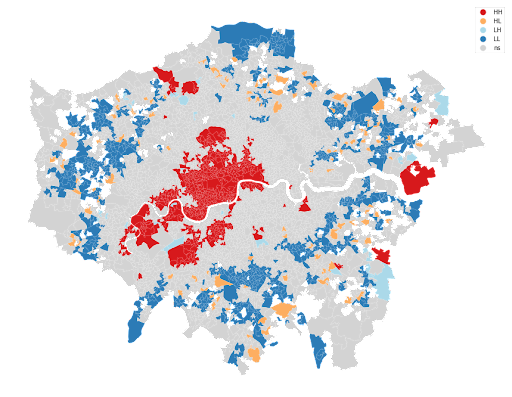
\includegraphics[width=0.65\textwidth]{2/figures/esda.png}
			\caption[Análisis Exploratorio de Datos Espaciales (ESDA)]{Análisis Exploratorio de Datos Espaciales (ESDA).\\
			Fuente: \cite{bk_haining2003spdat}. \citetitle{bk_haining2003spdat}. (p. 181)}
			\label{2:fig10}
		\end{center}
	\end{figure}
		

	\item \textbf{Modelos de Análisis Espacial}:para estimar y modelar el semivariograma, se presentan modelos de análisis espacial, como kriging con datos gaussianos que se muestra en la Figura 25. Esto es particularmente útil para datos de superficies continuos. \parencite{bk_haining2003spdat}
	
	\begin{figure}[h]
		\begin{center}
			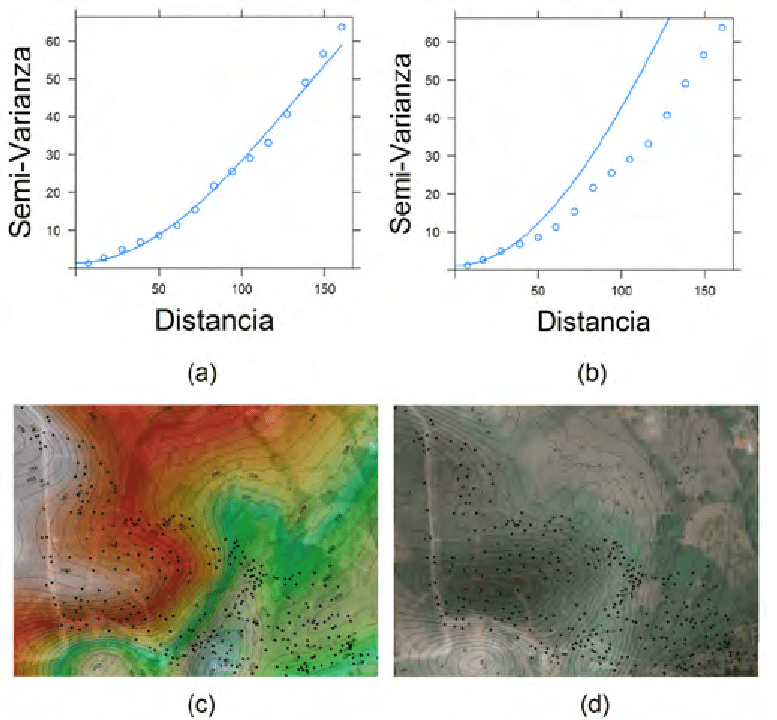
\includegraphics[width=0.70\textwidth]{2/figures/kriging.jpg}
			\caption[El modelo gaussiano isotrópico; el modelo gaussiano anisotrópico ajustado; la predicción de Kriging Simple Residual; y la varianza de Kriging Simple Residual.]{El modelo gaussiano isotrópico; el modelo gaussiano anisotrópico ajustado; la predicción de Kriging Simple Residual; y la varianza de Kriging Simple Residual.\\
			Fuente: \cite{bk_haining2003spdat}. \citetitle{bk_haining2003spdat}. (p. 352)}
			\label{2:fig11}
		\end{center}
	\end{figure}

	\item \textbf{Logistic Regression}: modela fenómenos espaciales como las relaciones entre variables espaciales y no espaciales. \parencite{bk_haining2003spdat}
	
	\begin{figure}[h]
		\begin{center}
			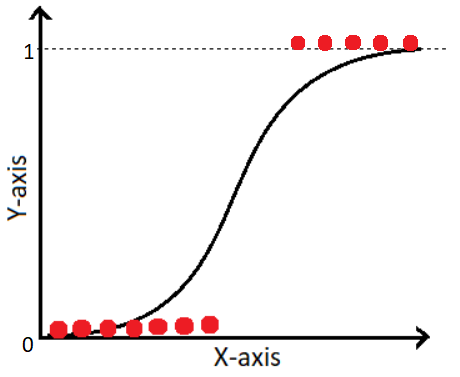
\includegraphics[width=0.70\textwidth]{2/figures/logisticregression.png}
			\caption[Regresión Logística]{Regresión Logística.\\
			Fuente: \cite{bk_haining2003spdat}. \citetitle{bk_haining2003spdat}. (p. 358)}
			\label{2:fig12}
		\end{center}
	\end{figure}
\end{itemize}
	
\subsection{Procesamiento del Lenguaje Natural}
El Procesamiento del Lenguaje Natural es un campo que involucra ciencias de la computación, lingüística computacional, ciencia cognitiva e inteligencia artística. Investiga cómo las computadoras pueden comprender el lenguaje humano para realizar tareas útiles y tener interacciones entre ambas partes. El reconocimiento de voz, la comprensión del lenguaje hablado, los sistemas de diálogo, el análisis léxico y el análisis de sentimientos son algunas de estas tareas. \parencite{bk_deng2018deeplearningnlp}.

En su libro, los autores \citeauthor{bk_deng2018deeplearningnlp} dividen el aprendizaje profundo, el racionalismo y el empiricismo en tres corrientes históricas.

\begin{itemize}
	\item \textbf{Racionalismo}: según los argumentos de Noam Chomsky sobre la concepción del lenguaje humano, una nomenclatura establecida entre las décadas de los 60s y 80s, se basa en el conocimiento humano, fijado por herencia genética y concebido desde el nacimiento. La aplicación inicial de esta estrategia se remonta a la década de los 50s, cuando Alan Turing realizó experimentos conocidos como "las pruebas de Turing" para simular conversaciones de lenguaje natural entre un humano y un computador para generar respuestas similares a las de una persona para poder evaluar sus habilidades. Los sistemas de entendimiento del lenguaje hablado y los sistemas de diálogo se basaron en conjuntos de reglas creados por la ingeniería de conocimiento experto durante las décadas de los 70s y 80s.

	\item \textbf{Empirismo}: se caracterizó por el uso de Aprendizaje Automático y la explotación del cuerpo de texto. Según esta noción, el cerebro humano comienza con operaciones de asociación, patrones de reconocimiento y generalización. El Modelo Ocultro de Markov (HMM) y los modelos de traducción de IBM son ejemplos.
	
	\item \textbf{Aprendizaje Profundo}: para resolver problemas de lengua natural que el Aprendizaje Automático no puede resolver en el aprendizaje con grandes cantidades de datos. Las Redes Neuronales Artificiales son las más populares porque su configuración permite personalizar su arquitectura basada en múltiples capas e hiperparámetros para soportar un gran entrenamiento. No obstante, a pesar de sus ventajas, existen ciertas limitaciones, como la falta de detalle para obtener impresionantes resultados estadísticos, una gran habilidad computacional o una falta de comprensión de las relaciones interoracionales, como frases o palabras progresivas dentro de una oración.
\end{itemize}

Los modelos mencionados anteriormente incluyen las Redes Neuronales Convolucionales (CNN) y las Redes Neuronales Recurrentes (RNN), que son algunas de las técnicas de aprendizaje profundo que se utilizan actualmente para resolver problemas de lenguaje natural. A continuación se describen algunos de los más comunes, junto con las principales características y diferencias de los ejemplos ya mencionados.

\begin{itemize}
	\item \textbf{Redes Neuronales Convolucionales}: Entre las técnicas de minería de datos, se explicaron los conceptos y tipos de Redes Neuronales Artificiales, entre ellas, la actual mencionada. Se comentó que entre sus mayores usos se dan actualmente en el tratamiento de imágenes, problemas de clasificación a partir de estas y visión por computador. El ejemplo más popular fue ImageNet desarrollado por Yann LeCun, informático reconocido por ser el fundador de este tipo de redes, para reconocer objetos dentro de imágenes.
	
	Pero también se utilizan para problemas de clasificación de texto. El uso de las CNN en tareas de procesamiento de lenguaje natural fue pionero por Ronan Collobert y Jason Weston, quienes modificaron su arquitectura y parámetros internos \parencite{bk_kamath2019deeplearning_nlp_sr}. La arquitectura de una CNN para problemas de procesamiento natural de la información se muestra en la Figura \ref{2:fig40}.
	\begin{figure}[!ht]
		\begin{center}
			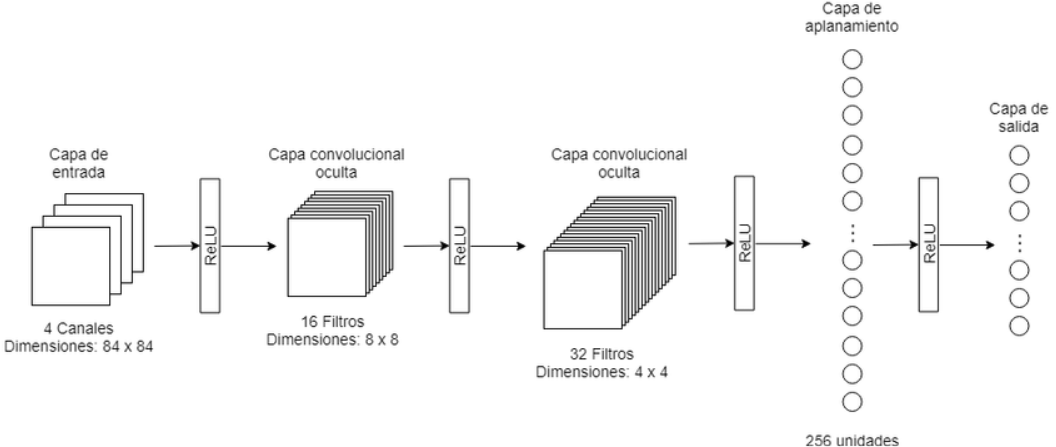
\includegraphics[width=0.95\textwidth]{2/figures/cnn_nlp.png}
			\caption[Arquitectura de un modelo CNN]{Arquitectura de un modelo CNN.\\
			Fuente: \cite{tec_kim2014convolutional}. \citetitle{tec_kim2014convolutional}. (p. 1747)}
			\label{2:fig40}
		\end{center}
	\end{figure}
	
	Las convoluciones de imágenes son bidimensionales (2d) porque se desplazan a través de matrices de dos dimensiones (largo y ancho), lo que es una de las principales diferencias entre ambos tipos de aplicaciones. Sin embargo, debido a que están conformadas por vectores y aprenden patrones en la dimensión de secuencia, las convoluciones unidimensionales (1d) son muy útiles para series de tiempo y operaciones de lenguaje natural \parencite{bk_rao2019nlp_pytorch}. La Figura \ref{2:fig41} muestra una comparación entre ambos tipos de convolución según el tamaño de dimensión.

	\begin{figure}[!ht]
		\begin{center}
			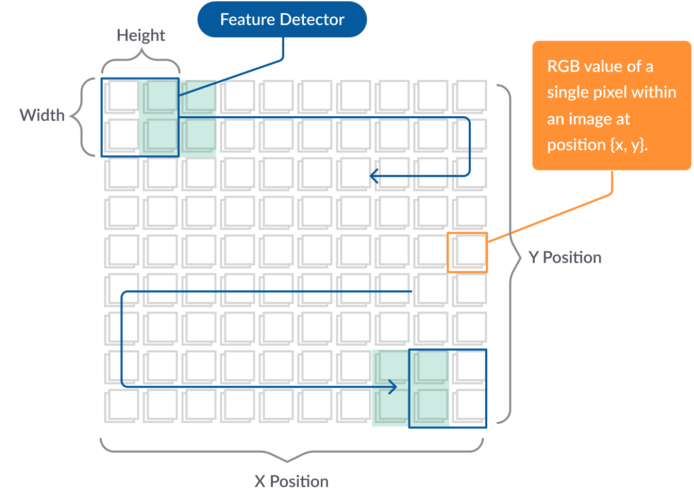
\includegraphics[width=0.95\textwidth]{2/figures/2D-convolutional-example.png}
			\caption[Diferentes dimensiones de convoluciones]{Diferentes dimensiones de convoluciones.\\
			Fuente: \cite{tec_missinglink_conv1d}. \citetitle{tec_missinglink_conv1d}.}
			\label{2:fig41}
		\end{center}
	\end{figure}

	En la imagen anterior, donde cada palabra codificada se representa por un vector, un núcleo de convolución de tamaño de 2 bloques (\textit{kernel\_size}) recorre toda la oración con un paso de 1 bloque (\textit{stride}).

	El proceso de la arquitectura CNN generalmente se basa para problemas de clasificación de texto como los que se consideran en esta investigación y en algunos antecedentes con contenido textual.
	
	La idea general es crear vectores de palabras codificadas para generar una matriz, que puede ser recorrida por filtros de una dimensión para generar mapas de características para la siguiente entrada. Para generar nuevos vectores univariantes de cada capa resultante, se agruparán según el criterio del usuario (puede ser el valor máximo, mínimo, promedio, etc.) y luego se concatenarán y luego el valor final de predicción regularizado entre un rango (dependiendo de la función de activación asignada para el problema para clasificación de 2 clases o de 3 clases).

	\item \textbf{Redes Neuronales Recurrentes}: los tipos de redes neuronales más conocidos también hablaron brevemente sobre este tipo de redes. Incluso en series de tiempo, las RNN son muy utilizadas porque los datos son secuencias, es decir, una colección ordenada de elementos. En el lenguaje humano, donde los fonemas son secuencias de palabras, se puede usar un elemento dependiente para predecir la siguiente palabra en una oración dada. En este ejemplo, las palabras previas \parencite{bk_rao2019nlp_pytorch}. Los motores de búsqueda en navegadores o sitios web, traductores, entre otros, son ejemplos de estos casos de uso más comunes.
	
	\item \textbf{Modelo Secuencia a Secuencia}: es un tipo de generador de lenguaje natural (textit Natural Language Generation o NLG) que se utiliza con frecuencia en la traducción. Se basa en dos capas LSTM, la primera de las cuales se utiliza para codificar la oración de entrada en un "vector de pensamiento", mientras que la segunda capa se utiliza para decodificar una respuesta (ver Figura \ref{2:fig46}), \parencite{bk_deng2018deeplearningnlp}.

	\begin{figure}[!ht]
		\begin{center}
			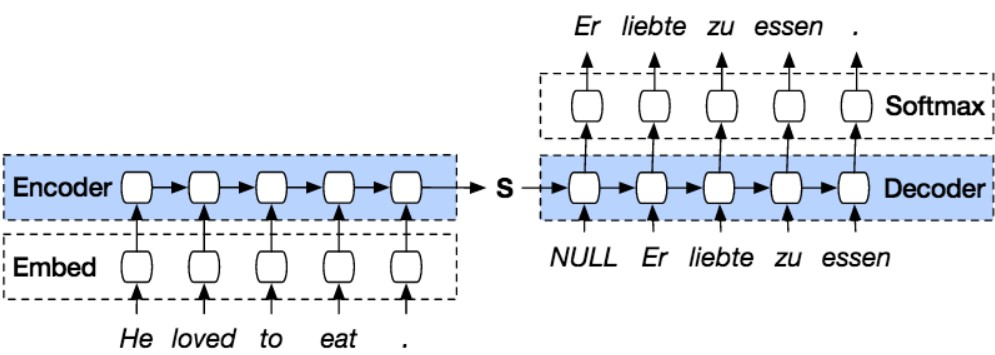
\includegraphics[width=0.67\textwidth]{2/figures/encoder-decoder.jpg}
			\caption[Arquitectura de un modelo Seq2seq]{Arquitectura de un modelo Seq2seq.\\
			Fuente: \cite{tec_kostadinov2019seq2seq}. \citetitle{tec_kostadinov2019seq2seq}.}
			\label{2:fig46}
		\end{center}
	\end{figure}	
\end{itemize}

Los modelos anteriores requieren un preprocesamiento del contenido textual. No se puede incluir el texto en su estado original en los modelos de aprendizaje automático o profundo sin previamente limpiarlo, según \parencite{bk_brownlee2017deeplearning_nlp}. Natural Language Toolkit, también conocida como NLTK, es una librería que Python proporciona para modelar y trabajar texto. Algunas de las funciones que están disponibles incluyen separar el texto en oraciones, separarlo en palabras o tokenizarlo, eliminar signos de puntuación, eliminar palabras de parada, reducir palabras a su forma raíz, volver palabras a su forma base o diccionario.

Suprimir contenido como signos de puntuación, caracteres especiales, palabras de parada, enlaces web, entre otros, ayuda a reducir la cantidad de vectores innecesarios para representaciones de palabras que se utilizan en la fase de entrenamiento. Para lograrlo, la secuencia de entrada debe dividirse en "tokens", que pueden ser una palabra, una oración o un párrafo.

Para la tokenización, NLTK ofrece varias opciones, como WhitespaceTokenizer (elimina espacios en blanco para separar palabras y signos de puntuación en una oración, que no son independientes), TreebankWordTokenizer (separa palabras y signos de puntuación en una oración de manera independiente) y WordPunctTokenizer (funciona como TreebankWordTokenizer pero no distingue contracciones en idiomas como el inglés). La elección de alguna de estas depende del propósito del usuario. Además, se pueden eliminar los sufijos o prefijos que se agregan a una palabra al reducir las palabras hacia su raíz, una técnica conocida como stem. Sin embargo, presenta problemas de manera irregular, produciendo "No palabras". El retorno de palabras a su forma original, también conocido como "lemma", convierte palabras conjugadas en diferentes variantes de tiempo. Sin embargo, no todas las formas se pueden reducir. Estos dos últimos tienen como objetivo reducir una palabra a su forma más primitiva (expresiones comunes) con el fin de crear un diccionario homogéneo, \parencite{tec_zimovnov2018text_preprocessing}.

Después de la limpieza de texto, el conjunto de datos recién creado debe representarse como vectores.

\newpage